\documentclass[american,]{article}
\usepackage{lmodern}
\usepackage{amssymb,amsmath,amsthm}
\usepackage{ifxetex,ifluatex}
\usepackage{fixltx2e} % provides \textsubscript
\ifnum 0\ifxetex 1\fi\ifluatex 1\fi=0 % if pdftex
  \usepackage[T1]{fontenc}
  \usepackage[utf8]{inputenc}
\else % if luatex or xelatex
  \ifxetex
    \usepackage{mathspec}
  \else
    \usepackage{fontspec}
  \fi
  \defaultfontfeatures{Ligatures=TeX,Scale=MatchLowercase}
\fi
% use upquote if available, for straight quotes in verbatim environments
\IfFileExists{upquote.sty}{\usepackage{upquote}}{}
% use microtype if available
\IfFileExists{microtype.sty}{%
\usepackage{microtype}
\UseMicrotypeSet[protrusion]{basicmath} % disable protrusion for tt fonts
}{}
\usepackage[margin=1in]{geometry}
\usepackage{hyperref}
\hypersetup{unicode=true,
            pdftitle={The reference model approach in feature selection problems},
            pdfauthor={Federico Pavone, Juho Piironen, Paul-Christian B\"{u}rkner, Aki Vehtari},
            pdfkeywords={keywords},
            pdfborder={0 0 0},
            breaklinks=true,
            colorlinks=true,
            linkcolor=black,
            citecolor=RoyalBlue,
            filecolor=black,
            urlcolor=RoyalBlue,
          }
\urlstyle{same}  % don't use monospace font for urls
\ifnum 0\ifxetex 1\fi\ifluatex 1\fi=0 % if pdftex
  \usepackage[shorthands=off,main=american]{babel}
\else
  \usepackage{polyglossia}
  \setmainlanguage[variant=american]{english}
\fi
\usepackage{natbib}
\bibliographystyle{plainnat}
\usepackage{placeins}
\usepackage{graphicx,grffile,subcaption}
\makeatletter
\def\maxwidth{\ifdim\Gin@nat@width>\linewidth\linewidth\else\Gin@nat@width\fi}
\def\maxheight{\ifdim\Gin@nat@height>\textheight\textheight\else\Gin@nat@height\fi}
\makeatother
% Scale images if necessary, so that they will not overflow the page
% margins by default, and it is still possible to overwrite the defaults
% using explicit options in \includegraphics[width, height, ...]{}
\setkeys{Gin}{width=\maxwidth,height=\maxheight,keepaspectratio}
\IfFileExists{parskip.sty}{%
\usepackage{parskip}
}{% else
\setlength{\parindent}{0pt}
\setlength{\parskip}{6pt plus 2pt minus 1pt}
}
\setlength{\emergencystretch}{3em}  % prevent overfull lines
\providecommand{\tightlist}{%
  \setlength{\itemsep}{0pt}\setlength{\parskip}{0pt}}
\setcounter{secnumdepth}{3}
% Redefines (sub)paragraphs to behave more like sections
\ifx\paragraph\undefined\else
\let\oldparagraph\paragraph
\renewcommand{\paragraph}[1]{\oldparagraph{#1}\mbox{}}
\fi
\ifx\subparagraph\undefined\else
\let\oldsubparagraph\subparagraph
\renewcommand{\subparagraph}[1]{\oldsubparagraph{#1}\mbox{}}
\fi

%%% Use protect on footnotes to avoid problems with footnotes in titles
\let\rmarkdownfootnote\footnote%
\def\footnote{\protect\rmarkdownfootnote}

%%% Change title format to be more compact
\usepackage{titling}

% Create subtitle command for use in maketitle
\newcommand{\subtitle}[1]{
  \posttitle{
    \begin{center}\large#1\end{center}
    }
}

\setlength{\droptitle}{-2em}

   
\usepackage{booktabs}
\usepackage{longtable}
\usepackage{array}
\usepackage{multirow}
\usepackage[table,dvipsnames]{xcolor}
\usepackage{wrapfig}
\usepackage{float}
\usepackage{colortbl}
\usepackage{pdflscape}
\usepackage{tabu}
\usepackage{threeparttable}
\usepackage{threeparttablex}
\usepackage[normalem]{ulem}
\usepackage{makecell}

\usepackage{soul}
\usepackage{mathtools}
\usepackage[utf8]{inputenc}
\usepackage[T1]{fontenc}
\usepackage{textcomp}
\usepackage{graphicx,pdflscape}
\usepackage{geometry}
\usepackage{amsmath}
\usepackage{float}
\usepackage{supertabular}
%\usepackage{booktabs,caption,fixltx2e}
\usepackage{booktabs,fixltx2e}
\usepackage[font={small,it}]{caption}
\usepackage{tcolorbox}
\usepackage{paralist}
\usepackage{multicol}
\setcitestyle{round}
\newcommand\numberthis{\addtocounter{equation}{1}\tag{\theequation}}
\theoremstyle{definition}
\newtheorem{example}{Example}


\title{The reference model approach in feature selection problems 
	\vspace{.1in}}
    \pretitle{\vspace{\droptitle}\centering\huge}
  \posttitle{\par}
  \author{Federico Pavone, Juho Piironen, Paul-Christian B\"{u}rkner and Aki Vehtari}
    
    \author{
    Federico Pavone, 
  Juho Piironen,
  Paul-Christian B\"{u}rkner
  and Aki Vehtari \footnote{Helsinki Institute for Information Technology HIIT,
  Department of Computer Science, Aalto University, Finland.}
  }
	 
    
    \preauthor{\centering\large\emph}
  \postauthor{\par}
    \date{\today}
    \date{\today}
%    \predate{}\postdate{}


\begin{document}
\maketitle
\begin{abstract}
When a reference model is used to guide the variable selection problem, it acts as a noise-filter modelling the data generation mechanism. We show how this translate into higher stability and better selection of variables. We devise a simple reference model approach that can be used on top of any feature selection procedure and use the normal means problem as a benchmark comparing different methods using or not a reference model. We include in our comparisons state-of-the-art complete selection procedures showing improved stability, false discovery rate and sensitivity of the selection, and also Bayesian methods controlling the amount of posterior shrinkage and bias. Furthermore we show in a real-world example the benefits achieved by the reference model through the projection predictive approach compared to the selection via stepwise backward regression.
\end{abstract}

\hypertarget{introduction}{%
\section{Introduction}\label{introduction}}

In statistical applications, one of the main steps in the modeling
workflow is covariate or feature selection, which is a special case of
model reduction. Variable selection may have multiple goals. 
First, if the covariates themselves are of interest,
we can use variable selection as an inferential tool to find the entire 
collection of variables which have some predictive information about the target variable.
Second, as simpler models come with the advantages of reduced
measurement costs and improved interpretability, we may be interested in
finding the minimal subset of covariates which
provides good predictive performance (or good balance between simplicity and
predictive performance). 
Whenever the predictive capability is guiding the selection, the true data generation
mechanism of future data can be approximated either by using the observed data directly or
alternatively by using predictions from a \emph{reference model}.

In data based approaches, such as Lasso selection
\citep{tibshirani1996regression} or stepwise backward/forward 
regression \citep{venables2013modern,harrell2015regression}, the observed empirical data distribution is utilized as a
proxy of future data usually in combination with cross-validation
or information criteria to provide estimates for out-of-sample
predictive performance.
In contrast, reference model based methods approximate the future data generation
mechanism using the predictive distribution of a reference model,
which can be, for example, a full-encompassing model including all
covariates. The reference
model approach has been used for long time in Bayesian statistics
since the seminal work of \citet{paper:reference_lindley}. For more
historical references, see the review by \citet{vehtari2012survey}, and for
most recent methodological development see 
\citet{paper:projpred}.
Reference models have been also used in non-Bayesian contexts,
where \cite{harrell2015regression} describes them as full models that
can be thought of as a ``gold standard'' (for a given application).
For example,
\cite{faraggi2001understanding} deal with the necessity of identifying
interpretable risk groups in the context of survival data using neural
networks, which typically perform very well in terms of prediction,
but whose covariates are difficult to be understood in terms of
relevance. 
\cite{paul2008preconditioning}, using the term preconditioning,
explore approximating models fitting Lasso or stepwise regression
against consistent estimates $\hat{y}$ of a reference model instead of
the observed responses $y$.

In this paper, we examine the benefits of using reference
models in detail. We illustrate how a properly designed reference model is able 
to filter parts of the noise present in the data, and hence provides an improved and more
stable selection process. This holds even if the reference model does not actually resemble the
true data generating process. Moreover, our analyses indicate that the substantial reduction of
variance attributable to noise is usually
more important than small potential bias due model misspecification.
We argue that, regardless of how the reference model is set up and used in the
inference procedure, it can be always seen as acting as a filter on the observed 
data. Following this idea, we devise a simple reference model approach that can
be applied on top of any variable selection procedure. 

In our simulations and analysis of real data, we apply several state-of-the-art methods for variable selection and compare,
for each of these methods, the results obtained by using a data based and a
reference model based approach. When a full 
variable selection is carried out, we report and compare quantities such as 
the false discovery rate \citep{paper:fdr_BH}, sensitivity and stability of the selection \citep{paper:stability}. For fully Bayesian methods, we additionally report results in terms of shrinkage and accuracy of the posterior estimates.
We show the benefits
of a reference model approach, regardless of what specific procedure is applied, using 
the normal means estimation problem as a benchmark. 
Variable selection is typically most challenging in 
\textit{small n large p} scenarios, that is, scenarios with small number of
observations but a lot of unknown model parameters. 
These occur frequently, for example, 
in microarray data analysis in medicine or biology \citep{dudoit2003multiple,liao2007logistic,paper:efron}.
In general, the less data we have and the more complex 
the estimated models, the higher the benefit of using a reference
models as the basis for variable selection.
Our results indicate that the core reason why the reference model based
methods perform well is the reference model itself, rather than the
specific way of using it. We do recognise that all these methods
diversify how the subset of variables is actually chosen and which
properties it has, thus it remains fundamental to investigate and
develop such different procedures. We want to note that, although we focus on
Bayesian approach in this paper, the benefits of the reference model 
approach can also be obtained in non-Bayesian settings.


The remainder of the paper is structured as follows. In Section \ref{reference-model-approach}, we review the concept of the reference model, its benefits with examples, including the projection predictive approach, and how it can be used as a filter on data in a simple way. In Section \ref{comparison}, we use different methods for feature selection comparing the selection results with and without using a reference model in the framework of the normal means problem. Finally, we end with a conclusion in Section \ref{conclusion}.


%In statistical applications, one of the main steps of the modelling workflow is covariate or feature selection, which can be seen as a special case of model reduction. From a full Bayesian perspective, when the goal of the analysis is to do prediction, no selection should be carried out and integration over all parameters uncertainties, i.e. posterior distributions, is the recommended procedure. In a high dimensional parameter space the choice of the prior plays an even more key role due to different difficulties that can rise, as computation burden and overfitting. In addition to that, sometimes collecting all the features for a future observation is not possible or too expensive. In order to solve or, at least, simplify these problems, different feature selection procedures have been proposed both in the frequentist and the Bayesian setting \cite[e.g. see][]{paper:feature_selection,vehtari2012survey,paper:model_selection}. Sometimes the task of the analysis is not prediction, but rather inference on which variables are substantially related to the phenomenon of interest. This typically happens in a \textit{small n large p} scenario, as in many microarray data analysis in medicine or biology. A very large number of genes is usually analysed in two groups of individuals labeled as \textit{positive} or \textit{negative} to some disease. The main goal of the analysis is to spot the subset of explanatory genes in order to perform further experiments \cite[see examples in][]{efron2012large}.

% The necessity of carrying out the selection arises from different problematics. Sometimes the leading objective of the analysis is to predict future observationgs, thus the main focus in building the model is on the predictive performance. Yet a high dimensional parameter space often leads to dangers as overfitting or other technical problems, as expensive costs to collect all the features for future observations or computational and memory burdens (e.g. when operating on limited resources), and thus a sparser representation of the model would be preferred. In addition to that, simpler models bring also advantages in terms of interpretability. Some other times,
% variable selection can be also seen as an inferential tool: the interest is on knowing which variables are meaningful, or relevant, in relation to the target variable of interest.
% This typically happens in a \textit{small n large p} scenario, as in many microarray data analysis in medicine or biology.

% A very large number of genes is usually analysed in two groups of individuals labeled as \textit{positive} or \textit{negative} to some disease; the goal is to spot the subset of explanatory genes in order to perform further experiments \cite[see examples in][]{efron2012large}.


% process is going to be based on assumptions regarding the ``true''
% data generation mechanism.  Making assumptions means making models,
% thus we identify two families of feature selection, or more in general
% model reduction, approaches depending on how the data generation
% mechanism is modelled: the data based and the reference model based
% ones.


% The reference model approach has been used for long time in the Bayesian framework, an example the pioneering work by \cite{paper:reference_lindley}. Following \cite{goutis1998model}, \cite{paper:original_proj} project the posterior distribution of the reference model in each candidate model by minimisation of the Kullback-Liebler divergence, and then select the smallest one with enough explanatory power avoiding any prior elicitation for the submodels. In the special case of candidate models being GLMs from the exponential family, the optimisation problem corresponds to the task of finding the maximum likelihood estimate using the expected pointwise predictions of the reference model instead of the observed target values. Different extensions have followed \cite{paper:original_proj}, as \cite{nott2010bayesian} that add an $l_{1}$ penalty to select the best approximating model and \cite{tran2012predictive}, who select the best approximating model by optimising the Kullback-Liebler divergence between the predictive distribution of the reference model and the approximating model plus an $l_{1}$ penalty on the submodel coefficients. A recent review of these methods together with some methodological improvements, as clustered projection and selection by comparison of a predictive performance utility, is given by \cite{paper:projpred}.


% and shows some examples of how it can be used to seek a sparser approximation. He highlights some of the benefits as the possibility to calculate the accuracy with which the submodel approximates the best model and the inheritance of the shrinkage when it is applied to the full model.

% \cite{faraggi2001understanding} propose to combine the benefits of the neural networks, which become what we call reference models, with the interpretability of regression trees, in order to provide a framework to make inferences about risk groups.

%\cite{harrell2015regression} includes also the possibility of using simple least squares for the approximating models as long as the target is the linear predictor of a full regression model \hl{CHECK}.
%\cite{paper:projpred} extend the projection algorithm with the clustered projection and choose the best model comparing the predictive performance of the explored submodels with the reference model one.
%\cite{paper:projpred} show in their experiments the benefits of the projection predictive approach in terms of predictive ability of the selected model and smaller size compared to other methods. It could be of interest to know how often a certain method includes non-relevant features. One could argue that such question can not have a general answer, because it depends both on the data and, when it is used, on the choice of the reference model. Moreover in real settings it is hard to define what relevant means, in most of the cases all the features have some level of relevance in term of prediction ability and thus the question looses of meaning.  However, it is still possible to simulate certain artificial scenarios and control which features are included. \cite{paper:model_selection} report results about the proportion of relevant and non-relevant features selected with different variable selection methods, showing overall better results in favour of the projection predictive approach. The explored submodels using the projection show also a higher performance and stability with respect to the compared methods, given the same submodel size.

% We hope that this work can increase
% the attractiveness on this family of methods and, therefore, it can be
% of interest to a large number of practitioners.


\hypertarget{reference-model-approach}{%
\section{Why the reference model helps}\label{reference-model-approach}}

The main assumption under any reference model approach is that we
operate in an $\mathcal{M}$-\textit{complete} framework
\citep{book:bernardo_smith,vehtari2012survey}. That is, we assume to be able to construct a model whose predictions reflect the best available description of the uncertainty of future data. In practice, this will often be the full-encompassing model
(including all models we consider having non-zero prior
probability as submodels) which has passed model checking and criticism \citep[see,
e.g.][]{gelman2013bayesian}. 
 
A good predictive model is able to filter parts of the noise present in the data. The noise is the main source of the instability and tends to obscure the relevance of the covariates in relation to the target variable of interest. Indeed, let us consider the following explanatory example taken from \cite{paper:projpred}. The data generation mechanism is
\begin{alignat}{2} \label{eq:simulated_data}
     &f\sim N(0,1) && \nonumber \\ 
     Y|&f\sim N(f,1) && \\
     X_{j}|&f \overset{iid}{\sim} N(\sqrt{\rho}f,1-\rho) \quad &&j=1,..,k \nonumber \\
     X_{j}|&f \overset{iid}{\sim} N(0,1) &&j=k+1,..,p \nonumber,
\end{alignat}
where $f$ is the latent variable of interest of which $Y$ is a noisy observation. The first $k$ covariates are strongly related to the target variable $Y$ and correlated among themselves. Precisely, $\rho$ is the correlation among any pair of the first $k$ covariates, whereas $\sqrt{\rho}$ and $\sqrt{\rho/2}$ are the level of correlation between any relevant covariate and, respectively, $f$ and $Y$. If we had an infinite amount of observations, the sample correlation would be equal to the true correlation between $X_j$ and $Y$. However, even in this ideal asymptotic regime, this  correlation would still remain a biased indicator of the true relevance of each covariate (represented by the correlation between $X_j$ and $f$) due to the intrinsic noisy nature of $Y$.

When using a reference model, we first obtain predictions for $f$ using all the covariates $\{X_{j}\}_{j=1}^{p}$ taking into account that we have only observed the noisy representation $Y$ of $f$. If our model is good, we are able to describe $f$ better than $Y$ itself can, which improves the accuracy in the estimation of the relevance of the covariates.  Figure \ref{fig:correlation} illustrates this process in the form of a scatter plot of (absolute) correlations of the covariates with $Y$ against the corresponding correlations with the predictions of a reference model (in this case the posterior predictive means of model \eqref{eq:ref_mod}; see Section \ref{simulated-data}). Looking at the marginal distributions, we see that using a reference model to filter out noise in the data, the two groups of features (relevant and non-relevant) can be distinguished much better than when the correlation is computed using the observed noisy data directly. 

\begin{figure}[tp]
  \centering
  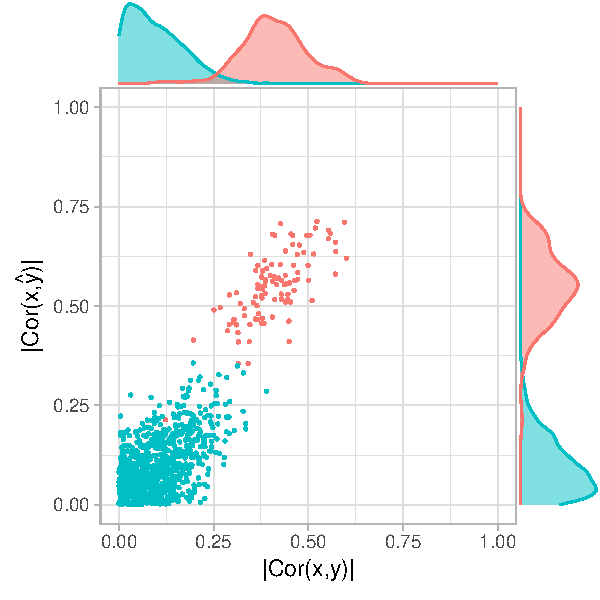
\includegraphics[width=0.3\textwidth]{graphics/correlation.pdf}
  \caption{Sample correlation plot of each feature (relevant in red, non-relevant in blue) with the target variable $y$ and the latent variable $f$ respectively on the x and y axis. Data are generated according to procedure \eqref{eq:simulated_data} with parameters $n=70$, $\rho=0.3$, $k=100$, $p=1000$.\\}
  \label{fig:correlation}
\end{figure}

% In Figure \ref{fig:correlation} the reference model filters the noise.
% This simple idea is what happens every time a reference model is used, as it is evident for example in the preconditioning by \cite{paul2008preconditioning} or in the draw-by-draw projection for GLMs by \cite{paper:original_proj}.\\
% Above the correlation was used to estimate the relevance of a covariate.  
As an another example, let us consider a candidate submodel in a feature selection process and let us refer to the parameter distribution of the submodel by $\pi$ and to the induced predictive distribution by $q_{\pi}(\tilde{y})$. We would like to choose $\pi$ so that $q_{\pi}(\tilde{y})$ maximises some predictive performance utility, for example, the expected log-predictive density (elpd) defined as:
\
\begin{equation}\label{eq:elpd}
\text{elpd}[q_{\pi}]=\int \text{log}\,q_{\pi}(\tilde{y})p_{t}(\tilde{y})d\tilde{y},
\end{equation}
where $p_{t}(\tilde{y})$ denotes the (usually unknown) true generating mechanism of future data $\tilde{y}$. If we refer to the posterior predictive distribution of a reference model with $p(\tilde{y}|D)$, where $D$ stands for the data on which we conditioned on, we can approximate \eqref{eq:elpd} using $p(\tilde{y}|D)$ instead of the true data generation mechanism $p_{t}(\tilde{y})$. The maximisation of the elpd using the reference model predictive distribution is equivalent to the minimisation of the KL divergence between the reference model's and the submodel's predictive distributions:
\
\begin{equation} \label{proj_as_filter}
\underset{\pi}{\text{max}} \; \int \text{log}\,q_{\pi}(\tilde{y})p(\tilde{y}|D)d\tilde{y} \leftrightarrow \underset{\pi}{\text{min}} \; \text{KL}[p(\tilde{y}|D)||q_{\pi}(\tilde{y})] 
\end{equation}
The term on the right-hand side of Equation \eqref{proj_as_filter} describes what is referred to as the projection of the predictive distribution, which is the general idea behind the projection predictive approach (cite). Again the reference model is acting as a filter, or substitute, on data.

%--- OR ---

%What we do in Figure \ref{fig:correlation} is to use the reference model predictive ability as a noise-filter on the observed data. This simple idea is what happens every time a reference model is used, as it is evident for example in the preconditioning by \cite{paul2008preconditioning} or in the draw-by-draw projection for GLMs by \cite{paper:original_proj}. Also the general idea of the projection of the predictive can be seen under this perspective. Indeed, let us call $p_{\text{ref}}(\tilde{y}|D)$ the posterior predictive distribution for a new observation $\tilde{y}$ for the reference model and let $\pi(\theta)$ and $q_{\pi}(\tilde{y})$ be respectively the submodel parameter and the induced predictive distributions. The projection of the predictive distribution allows to find the optimal parameter distribution $\pi^{*}$ minimising the KL discrepancy among the induced predictive distribution of the submodel and the reference model one:
%\
%\begin{equation} 
%\pi^{*}\quad \text{s.t.} \quad \text{KL}[p_{\text{ref}}(\tilde{y}|D)||q_{\pi^{*}}(\tilde{y})]=\underset{\pi}{\text{min}} \; \text{KL}[p_{\text{ref}}(\tilde{y}|D)||q_{\pi}(\tilde{y})] 
%\end{equation}
%Consider now the predictive performance of such submodel, a common utility in Bayesian context is the expected log-predictive density defined as:
%\
%\begin{equation} 
%\text{elpd}[q_{\pi}]=\int \text{log}\,q_{\pi}(\tilde{y})p_{t}(\tilde{y})d\tilde{y} 
%\end{equation}
%where $p_{t}$ is the distribution of a new observation under the true data generation mechanism. Maximising the elpd of a model is equivalent to minimising the KL-divergence of its predictive distribution from the true data generation mechanism. Therefore the projection corresponds to maximising the elpd using as distribution of the true data generation mechanism the posterior predictive distribution of the reference model, i.e.:
%\
%\begin{equation} \label{proj_as_filter}
%\underset{\pi}{\text{min}} \; \text{KL}[p_{\text{ref}}(\tilde{y}|D)||q_{\pi}(\tilde{y})] \leftrightarrow \underset{\pi}{\text{max}} \; \int \text{log}\,q_{\pi}(\tilde{y})p_{\text{ref}}(\tilde{y}|D)d\tilde{y} 
%\end{equation}
%Equation \eqref{proj_as_filter} clearly shows the action of the reference model as a filter on our target observations, substituting the unknown true data generation mechanism, that is usually estimated with the data empirical distribution, with the best known approximation that is available, i.e. the reference model posterior predictive distribution.

%------------------

Relying on the idea of the reference model as a noise-filter, a generic reference model approach, which can be used on top of any feature selection procedure, consists of simply substituting the target observations with corresponding point predictions of the reference model, for instance, the posterior predictive means. Afterwards, any method for feature selection can be used. Note that we do not argue that such a reference model approach should necessarily be used as is for feature selection in real applications. There are several more sophisticated reference model approaches available in the literature (cite), which are likely to yield even better results. Rather, the reason for focussing on this simple version is to enable a fair comparison between a reference model and a purely data based approach when otherwise using the same selection procedures. Other kinds of comparisons, as the one presented in Section \ref{projection}, work well as motivational examples but fail in terms of generality since the presence or absence of a reference model is not the only aspect differentiating the two procedures. We will come back to the more general comparison in Section \ref{comparison}.

%we compare some well-known methods from the literature using both such reference model approach and the original data, observing at the end of the selection higher stability and quality of the selection thanks to the reference model.

\hypertarget{projection}{%
\subsection{Benefits of the reference model: an example with the projection predictive approach}\label{projection}}

As a motivational example to the implications of using a reference model in feature selection problems, we show its application in the form of the projection predictive approach, which uses the reference model to project the posterior samples to the submodels (cite). The \texttt{R}-package \texttt{projpred} (available at \url{https://CRAN.R-project.org/package=projpred}) implements the projection in case of submodels in the family of the generalised linear models and, additionally, it provides a framework to choose the optimal submodel size through a predictive utility comparison between the submodels and the reference model. 
\\
We now summarise the workflow of the projection predictive approach in the particular case of the draw-by-draw projection \cite[original formulation by][]{paper:original_proj}, following \cite{paper:projpred}. Suppose we have observed $n$ statistical units with target values $\{y_{i}\}_{i=1}^{n}$ and a set of observed covariates for which we want to obtain a minimally relevant subset. Than, the main steps are the following:
\begin{enumerate}
\item Devise and fit a reference model. Let $\{\boldsymbol{\theta}_{*}^{s}\}_{s=1}^{S}$ be the set of $S$ posterior samples of the reference model's parameters.
\item Rank the covariates according to their relevance using some heuristics and consider as candidate submodels only those which preserve this order,  starting from including only the highest ranked covariate (the submodels are then naturally identified by their model size). This is not strictly necessary but reduces the number of submodels to consider in the following steps.
\item For each submodel, project the reference model's samples as follows:
\begin{equation}\label{eq:draw_by_draw}
\boldsymbol{\theta}_{\perp}^{s} = \underset{\boldsymbol{\theta^{s}}\in\Theta}{\text{argmin}} \frac{1}{n}\sum_{i=1}^{n}\text{KL} \left( p(\tilde{y}_{i}|\boldsymbol{\theta}_{*}^{s})\;||\;q(\tilde{y}_{i}|\boldsymbol{\theta}^{s}) \right) \quad s=1,..,S
\end{equation}
where $p(\tilde{y}_{i}|\boldsymbol{\theta}_{*}^{s})$ stands for the predictive distribution of the reference model with parameters fixed at the posterior sample $\boldsymbol{\theta}_{*}^{s}$ and conditioning on all the covariate values related to the statistical unit (identified by the subscript $i$), whereas $q(\tilde{y}_{i}|\boldsymbol{\theta}^{s})$ is the predictive distribution of the submodel. The projected samples $\boldsymbol{\theta}_{\perp}^{s}$ then correspond to the submodel's parameter distribution.
\item For each submodel (size), test the predictive performance for instance via cross-valdiation.
\item Choose the smallest submodel (size) that is sufficiently close to the reference model's predictive utility score.
\end{enumerate} 

Expression \eqref{eq:draw_by_draw} is not an easy optimisation problem in general, but in the special case of submodels for the family of generalize lineder models, \eqref{eq:draw_by_draw} reduces to a maximum likelihood estimation problem, which can be easily optimised (cite). For further details on the projective prediction workflow and implementation see \cite{paper:projpred}.

We show the benefits of the reference model in the form of the projection approach (projpred) with respect to the stepwise backward regression (steplm) using the body fat data \citep{johnson1996fitting}. The analysis is based on Vehtari's \texttt{R}-notebook available at \url{https://avehtari.github.io/modelselection/bodyfat.html}, which is inspired by \cite{paper:bodyfat}. The target variable of interest is the amount of body fat, which is measured with a complex and expensive procedure. Additionally, we have information about 13 covariates which are anthropometric measurements (e.g., height and weight), some of which are highly correlated among themselves and thus provide some challenges in the model selection. In total, we have 251 observations. The goal is to find the simplest model which is able to predict the amount of fat sufficiently well. We use the same data again later on in Section \ref{real-world-data}.

\cite{paper:bodyfat} report results using steplm with a significance level of 0.157 with AIC selection, fixing abdomen and height to be always included in the model. Here, we implement steplm via AIC without fixing any variable. For selection via projpred, the reference model includes all the covariates, we regularize model complexity with a regularised horseshoe prior on the covariate coefficients (cite), submodels are explored using forward search, and the predictive utility is the expected log-predictive density (elpd) estimated using PSIS-LOO \citep{paper:psis_loo}. The experiments are implemented in \texttt{R} (cite). The steplm approach is carried out combining the \texttt{step} and \texttt{lm} functions, whereas the selection via projpred is done with the \texttt{projpred} package. In order to automatise the latter, we select the submodel as the one with the smallest size which has an elpd score higher (i.e., better) than the reference model score with probability of at least 5\%. The inclusion frequencies of each feature in the final model after 100 bootstrap samples are depicted in Figure \ref{fig:inclusion_frequencies}. The projpred approach has only two variables, 'abdomen' and 'weight', with inclusion frequencies above 50\% ('abdomen' is the only included always), the third most included is `wrist' at 44\%, and the fourth is `height' at 35\%, while steplm has seven features above 50\%. Such a lower stability of steplm can be observed also in the bootstrap model selection frequencies reported in Table \ref{tab:model_frequencies}. For exaple, the first five selected models have a cumulative frequency of 76\% with projpred, but only of 14\% with steplm. In addition, we note that the size of the selected model is much smaller when using projpred.

\begin{figure}[tp]
  \centering
  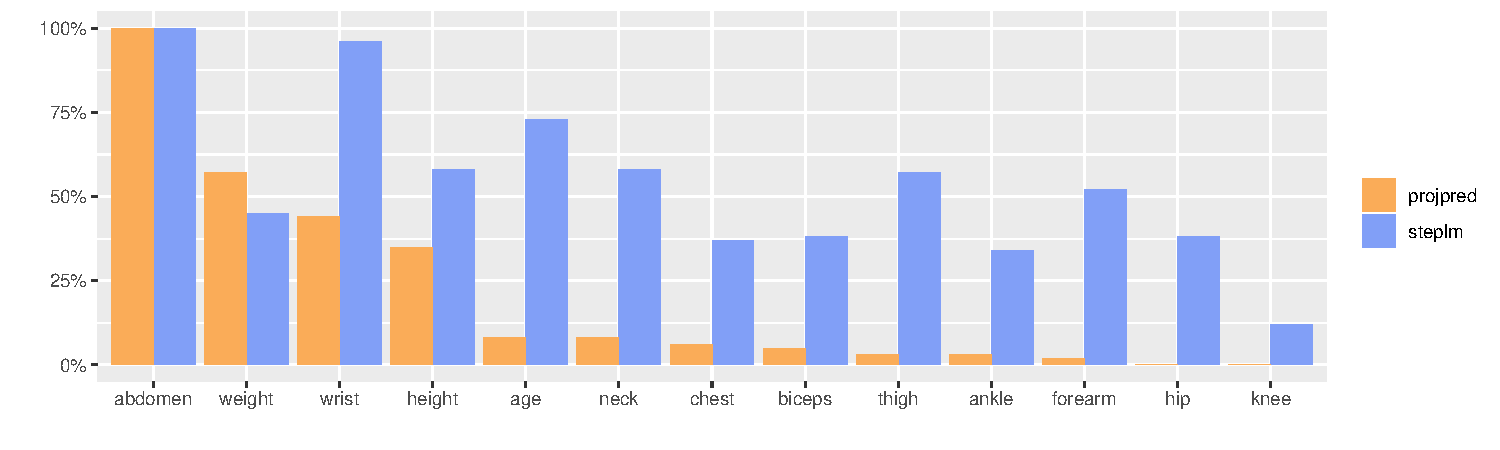
\includegraphics[width=0.98\textwidth]{graphics/inc_prob.pdf}
  \caption{Bootstrap inclusion frequencies after 100 bootstrap samples.}
  \label{fig:inclusion_frequencies}
\end{figure}


\begin{table}[tp]
\scriptsize
\centering
\begin{tabular}{l||l|r||l|r}
  \hline
M & projpred & Freq (\%) & steplm & Freq (\%)  \\ 
  \hline
1 & abdomen, weight & 39 & abdomen, age, forearm, height, hip, neck, thigh, wrist & 4 \\
2 & abdomen, wrist & 10 & abdomen, age, chest, forearm, height, neck, thigh, wrist & 4 \\
3 & abdomen, height & 10 & abdomen, forearm, height, neck, wrist & 2 \\
4 & abdomen, height, wrist & 9 & abdomen, forearm, neck, weight, wrist & 2 \\
5 & abdomen, weight, wrist & 8 & abdomen, age, height, hip, thigh, wrist & 2 \\
6 & abdomen, chest, height, wrist & 2 & abdomen, age, height, hip, neck, thigh, wrist & 2 \\
7 & abdomen, biceps, weight, wrist & 2 & abdomen, age, ankle, forearm, height, hip, neck, thigh, wrist & 2 \\
8 & abdomen, height, weight, wrist & 2 & abdomen, age, biceps, chest, height, neck, wrist & 2 \\
9 & abdomen, age, wrist & 2 & abdomen, age, biceps, chest, forearm, height, neck, thigh, wrist & 2 \\
10 & abdomen, age, height, neck, thigh, wrist & 2 & abdomen, age, ankle, biceps, weight, wrist & 2 \\
   \hline
\end{tabular}
\caption{Bootstrap model selection frequencies after 100 bootstrap samples.}
\label{tab:model_frequencies}
\end{table}


%\begin{table}[tp]
%\scriptsize
%\centering
%\begin{tabular}{l||l|r||l|r}
%  \hline
%M & projpred & Freq (\%) & steplm & Freq (\%)  \\ 
%  \hline
%1 & abdomen, weight & 34.2 & abdomen, height, wrist, age, chest, biceps & 3.2 \\
%2 & abdomen, wrist & 13.3 & abdomen, height, wrist, age, neck, forearm, thigh, hip & 2.9 \\
%3 & abdomen, weight, wrist & 7.6 & abdomen, height, wrist, age, forearm, chest & 1.9 \\
%4 & abdomen, height & 7.4 & abdomen, height, wrist, age, neck, forearm, chest & 1.9 \\
%5 & abdomen, height, wrist & 6.7 & abdomen, height, wrist, age, neck, forearm, chest, thigh, hip & 1.9 \\
%6 & abdomen, age, wrist & 2.9 & abdomen, height, wrist, age, neck, chest, biceps & 1.8 \\
%7 & abdomen, height, neck & 2.2 & abdomen, height, wrist, age, neck, thigh, biceps, hip & 1.6 \\
%8 & abdomen, age, height, wrist & 1.2 & abdomen, height, wrist, age, neck, forearm & 1.5 \\
%9 & abdomen, weight, thigh & 1.1 & abdomen, height, wrist, age, neck, biceps & 1.5 \\
%10 & abdomen, weight, neck & 1.0 & abdomen, height, wrist, age, beck, forearm, chest, biceps & 1.4 \\
%   \hline
%\end{tabular}
%\caption{Bootstrap model selection frequencies after 1000 bootstrap samples.}
%\label{tab:model_frequencies}
%\end{table}

Table \ref{tab:model_performances} reports the predictive performances, in terms of root mean square error, of the full model and the corresponding selected submodel using both projpred and steplm. We also repeat the selection after adding truely uncorrelated (i.e., irrelevant) features up to a total of 100 covariates. For this experiment, we report both the size of the selected submodel and the number of selected irrelevant features. Whilst, with the original data, we do not observe any gain using projpred in terms of predictive performance, what we do observe is a smaller size for the selected submodel, at the cost of a higher computation time compared to steplm. However, when additional irrelevant features are added, projpred is able to notably improve the predictive performance keeping the same submodel size, whereas steplm selects a much larger submodel also including a large number of irrelvant features (13 irrelevant out of a total of 19 selected features).

\begin{table}[tp]
\scriptsize
\centering
\begin{tabular}{l|r|r|r|r}
  \hline
 & RMSE(Full) & RMSE(Sel) & Size(Sel) & SizeIr(Sel) \\ 
  \hline
projpred & 4.35 & 4.47 & 2 & -  \\
steplm & 4.38 & 4.47 & 7 & - \\
\hline
\hline
projpred & 4.58 & 4.54 & 2 & 0  \\
steplm & 5.89 & 5.43 & 19 & 13 \\
   \hline
\end{tabular}
\caption{Model predictive performances with original data (first two rows) and adding noisy features (last two rows) estimated with 10-fold cross-validation. Abbreviations: Full = full model; Sel = selected submodel; Size = total number of included covariates; SizeIr = number of included irrelevant covariates.}
\label{tab:model_performances}
\end{table}

%\begin{table}[tp]
%\scriptsize
%\centering
%\begin{tabular}{l|r|r|r|r}
%  \hline
% & rmse.full & rmse.sel & size.sel & noisy.sel \\ 
%  \hline
%projpred & 4.4 & 4.5 & 2 & -  \\
%steplm & 4.4 & 4.5 & 7 & - \\
%\hline
%\hline
%projpred & $^{*}$4.4 & $^{*}$4.5 & 2 & 0  \\
%steplm & 5.3 & 5.5 & 38 & 32 \\
%   \hline
%\end{tabular}
%\caption{Model predictive performances with original data (first two rows) and adding noisy features (last two rows). Results with an asterisk using 10-fold CV, otherwise 20-fold CV.}
%\label{tab:model_performances}
%\end{table}

\hypertarget{computational-burden}{%
\subsection{Computational burden} \label{computational-burden}}

We consider the reference model approach as a family of methods, thus providing a general answer to the question of computational burden is not possible because not unique. It is possible to identify a common and inevitable overhead, though, which is the cost of fitting the reference model. In the simple ''bare-bones'' reference model approach we have described above, it is actually the only added cost. In general, a full Bayesian model is advisable in order to have the best predictive performance. However, including all the available features can often be quite computationally demanding. In such a case, a first possible speed-up could be using screening or dimensionality reduction techniques, as for example the supervised principal components \citep{bair2006prediction,piironen2018}. However, in some cases, this does not always result in an appreciable speed-up. For example, when there are several predictive but mutually uncorrelated features, all of them  have to be included in the reference model anyway. Other alternatives could be fixing some parameters to their maximum marginal likelihood value (typically referred as empirical Bayes; cite) or use a completely frequentist approach, if predictions are good enough.

The comparison example between projpred and steplm shows that such additional computational burden can be worth it. We found that the reference model approach (projpred) selected much sparser submodels, which can result in saving time and general costs using the selected model for future predictions. Table \ref{tab:model_performances} displays that there could even be an improvement in the predictive ability compared to the full model, thus justifying more additional computational costs in the selection procedure. More benefits obtainable through a reference model approach are provided in the experiments discussed in the upcoming section.


\hypertarget{comparison}{%
\section{A comparison in the normal means problem framework}\label{comparison}}

In this Section we show the benefits of the use of a reference model using as a benchmark the normal means estimation problem, which consists in estimating the vector of means, usually sparse, of a normal vector of observations. Let us call $p$ the dimensionality of the vector of means and let $\{z_{j}\}_{j=1}^{p}$ be the vector of observations of the random variables $\{Z_{j}\}_{j=1}^{p}$, the normal means problem consists in estimating the latent variables $\{\theta_{j}\}_{j=1}^{p}$ of the following model:
\
\begin{equation}\label{eq:normal_means_problem}
Z_{j}|\theta_{j},\sigma\overset{ind}{\sim}N(\theta_{j},\sigma^{2}) \quad j=1,..,p
\end{equation}
Note that it is equivalent to a linear regression where the design matrix is the identity one. This formulation can be retrieved in different ways, a common example is given by microarray data, where a large set of genes are usually tested in two groups of patient labelled as positive or negative to some disease. The objective of the analysis is to spot the whole subset of statistically relevant genes to the disease and one possible way to proceed is to compute the two-samples $t$-statistics for each gene and after combining it with the cumulative density function of the standard distribution, the resulting data can be used in the problem formulation \eqref{eq:normal_means_problem}. For further details see the examples in \cite{paper:efron, efron2012large}. 
\\
In our examples we retrieve the normal means problem from the sample correlation using the Fisher $z$-transformation approximation \citep{hawkins1989using}. Suppose to have a continuous target random variable $Y$ and a set of $p$ continuous covariates $\{X_{j}\}_{j=1}^{p}$ and let us call $\rho_{j}=Cor(Y,X_{j})$. Suppose to observe $n$ statistical units and define $r_{j}$ the sample correlation between the observations of the target variables $\{y_{i}\}_{i=1}^{n}$ and the j-th covariate $\{x_{ij}\}_{i=1}^{n}$. Let finally refer to the function $\text{tanh}^{-1}(\cdot)$ as $T_{F}(\cdot)$. It holds the following modelling approximation (assuming each pair $(Y,X_{j})$ normally distributed):
\
\begin{equation} \label{eq:fisher_transformation}
T_{F}(r_{j})\overset{ind}{\sim} N(T_{F}(\rho_{j}),\frac{1}{n-3}) \quad j=1,..,p
\end{equation}
Therefore rescaling the quantities $T_{F}(r_{j})$ by $\sqrt{n-3}$ and referring to the results as variables $z_{j}$, we find again formulation \eqref{eq:normal_means_problem} with unit variance:
\
\begin{equation} \label{eq:normal_means_problem2}
Z_{j}|\theta_{j}\overset{ind}{\sim}N(\theta_{j},1) \quad j=1,..,p
\end{equation}
Note that now the quantity of interest $\theta_{j}$ stands for $\sqrt{n-3}\,T_{F}(\rho_{j})$. There are different ways to proceed with the selection from the normal means problem, we consider in our comparison both frequentist and Bayesian state-of-the-art methods. From a full-Bayesian perspective, a Bayesian regression model is fitted to the normal means problem typically using a sparsifying prior as in \cite{paper:dirichlet_laplace}, \cite{bhadra2017horseshoe+} and \cite{johnstone2004needles}. In case of continuous priors, as the Dirichlet-Laplace (DL) and the horseshoe+ priors, there is not a canonical way to complete the selection since the posterior probability of an exactly zero signal is always zero; in their experiments \cite{paper:dirichlet_laplace} use k-means clustering over the posterior samples using the DL prior, whereas \cite{bhadra2017horseshoe+} focus the analysis on the obtained shrinkage and the correct estimation of the sparse signals using the horseshoe+ prior. We include in our experiments the DL prior and the regularised horseshoe (RHS) prior \citep{paper:rhs}, which has shown in our opinion better scalability with respect to the horseshoe+, comparing the shrinkage and the correct estimation of the sparse signals using or not the reference model approach. The quantity of interests that we consider are the average SSE (sum of square errors) and the average SESE (sum of expected square errors), defined as follows:
\
\begin{align}
\text{SSE}&=\frac{1}{n-3}\sum_{j=1}^{p}(\hat{\theta}_{j} - \theta^{0}_{j})^{2} \label{eq:SSE} \\
\text{SESE}&=\frac{1}{n-3}\sum_{j=1}^{p}\int_{\mathbb{R}}(\theta_{j}-\theta^{0}_{j})^{2}p(\theta_{j}|z_{1},..,z_{p})d\theta_{j} \\
&=\frac{1}{n-3}\sum_{j=1}^{p}\mathbb{E}_{\theta_{j}}[(\theta_{j}-\theta^{0}_{j})^{2}|z_{1},..,z_{p}] \label{eq:SESE}
\end{align}
where $\theta_{j}^{0}=\sqrt{n-3}\,T_{F}(\rho_{j})$ is the true value, $\hat{\theta}_{j}$ is the posterior median of each parameter $\theta_{j}$ and \eqref{eq:SESE} is a sum of posterior expectations. We divide the errors by $(n-3)$ to have quantities independent from the number of statistical units. Note that the quantity SESE takes in account also the uncertainty, thus the shrinkage, of the posterior distributions, whereas the SSE measures only the bias in the point estimates. Note also that any kind of point estimate could be used to compute the SSE, here we follow \cite{paper:dirichlet_laplace} using the posterior median. The results that we show later in Section \ref{shrinkage-signal} are not sensible to such a choice. We also take into account the posterior mean for the shrinkage factor ($\kappa_{j}$) for each parameter $\theta_{j}$, which for model \eqref{eq:normal_means_problem2} with a hierarchical shrinkage prior of the type:
\begin{align}
Z_{j}|&\theta_{j}\overset{ind}{\sim}N(\theta_{j},1) \qquad j=1,..,p \\
&\theta_{j}|\tau,\nu_{j}\overset{ind}{\sim}N(0,\nu_{j}^{2}\tau^{2})
\end{align}
is defined as:
\begin{equation}
\kappa_{j}=\frac{1}{1+\tau^{2}\nu_{j}^{2}}
\end{equation}
\
and, thus, in our case it becomes:
\begin{equation}
\kappa_{j}^{\text{RHS}}=\frac{1}{1+\tau^{2}\lambda_{j}^{2}}, \qquad \kappa_{j}^{\text{DL}}=\frac{1}{1+\psi\phi_{j}^{2}\tau^{2}}
\end{equation}
respectively for the regularised horseshoe and the Dirichlet-Laplace priors. In the left hand-side expression, $\tau$ and $\lambda_{j}$ stand for the global and local shrinkage parameters of the regularised horseshoe prior \cite[notation and further details in][]{paper:rhs}, whereas on the right hand-side $\psi\phi_{j}^{2}\tau^{2}$ is the variance term of the Dirichlet-Laplace prior of parameter $\theta_{j}$, following the same notation as \cite{paper:dirichlet_laplace}.


\cite{johnstone2004needles} use a prior of spike-and-slab type \citep{paper:spike_slab_mitchell} given by a mixture of a delta distribution in zero and a heavy-tailed distribution; when the latter is a Laplace distribution they show an interesting thresholding property of the median estimator and, thus, present a complete selection procedure using their prior. We include in our comparison such method (EB.med) together with the control of the local false discovery rate \cite[loc.fdr; see][]{efron2012large, paper:efron} and a simple selection procedure using inclusion probability at 0.9 for posterior credible intervals using the regularised horseshoe prior (ci.90). All these methods provide a complete selection procedures, we compare the result using or not a reference model on top of the procedure evaluating the average false discovery rate (i.e. ratio of the number of non-relevant selected features over the number of selected features) and the average sensitivity (i.e. ratio of the number of relevant selected features over the total number of relevant features). We also provide a comparison of the stability of the selection using the measure proposed by \cite{paper:stability}. Table \ref{tab:comparison} summarises the methods used in the comparison.

\begin{table}[tp]
\scriptsize
\centering
\begin{tabular}{l|l|l|l}
  \hline
 Method & Alias & Type & Quantities of interest \\ 
  \hline
 Regularised Horseshoe & RHS & Shrinkage prior & SSE, SESE, $\kappa$ \\
 Dirichlet-Laplace & DL & Shrinkage prior & SSE, SESE, $\kappa$ \\
 Local false discovery rate & loc.fdr & Complete selection & fdr, sensitivity, stability \\
 Median estimator & EB.med & Complete selection & fdr, sensitivity, stability \\
 Credible intervals & ci.90 & Complete selection & fdr, sensitivity, stability \\
 \hline
\end{tabular}
\caption{Summary of the methods used in the comparison.}
\label{tab:comparison}
\end{table}

\hypertarget{simulated-data}{%
\subsection{Simulated data}\label{simulated-data}}

Here we use simulated data in order to control the difficulty of the selection problem. We rely on the scheme \eqref{eq:simulated_data} using different levels of correlation ($\rho$) and number observation ($n$), precisely $p$ and $k$ are fixed respectively at $1000$ and $100$, whereas $n\in\{50,70,100\}$ and $\rho\in\{0.3,0.5\}$. Lower the correlation level and the number of observations are, more challenging the selection is. As mentioned, this data generation mechanism was already proposed by \cite{paper:projpred}, who also devise a reference model sufficiently good in predictions. It consists in a linear regression using the first five supervised principal components (SPCs) \citep{bair2006prediction, piironen2018} as follows:
\
\begin{equation}
\label{eq:ref_mod}
\begin{aligned}
    Y_{i}|&\boldsymbol{\beta},\sigma^{2},\boldsymbol{u}_{i} \overset{ind}{\sim} N(\boldsymbol{u}_{i}^{T}\boldsymbol{\beta},\sigma^{2}) \quad &i=1,..,n \\
    &\beta_{j}|\!\begin{aligned}[t] &\tau \overset{iid}{\sim} N(0,\tau^{2})\\
    &\tau \sim t_{4}^{+}(0,s_{max}^{-2}) 
    \end{aligned} &j=1,..,5 \\ 
    &\sigma \sim t_{3}^{+}(0,10) \\
\end{aligned}
\end{equation}
where $u_{ij}$ stays for the $j$-th SPC of observation $i$, and $s_{max}$ denotes the sample standard deviation of the largest SPC. We use as screening threshold for the SPCs the value $0.6s_{max}$, which has shown satisfying predictive performance. In our experiments the results are not very sensible to the chosen value, yet a more principled approach would be to use cross-validation to select the threshold as in \cite{paper:projpred}.
\\
The normal means problem formulation is obtained as explained in Section \ref{comparison} by Fisher-transformation. We label as ``ref'' the reference approach, which consists in using the reference model on top of the computation of the z-values, and ``data'' the standard approach based on the observed data only. In Section \ref{shrinkage-signal} we analyse in the context of full-Bayes methods the different shrinkage and signal estimation provided by the use of a reference model or not. Section \ref{complete-selection} shows results for the complete selection procedures.

\hypertarget{shrinkage-signal}{%
\subsubsection{Shrinkage and signal analysis}\label{shrinkage-signal}}
In the framework of full-Bayes methods we analyse the effect of the reference model using two continuous hierarchical shrinkage priors: the Dirichlet-Laplace \citep{paper:dirichlet_laplace} and the regularised horseshoe prior \citep{paper:rhs}. 
% Although the horseshoe+ prior by \cite{bhadra2017horseshoe+} is a state-of-the-art prior for sparse signal analysis in the context of the normal means problem, we decided to include the regularised horseshoe due to its faster MCMC inference, since our purpose in this paper is not to study the best prior choice, but rather compare and show the benefits of using a reference model when carrying out variable selection.
We used an uniform prior on the interval $(1/p,1/2)$ for the Dirichlet hyperparameter of the Dirichlet-Laplace prior, whereas regarding the reguelarised horseshoe prior we followed the indication provided in \cite{paper:rhs}, setting the prior guess of the effective number of parameters equal to 1 to achieve the highest shrinkage. Yet we have not observed any sensibility of the results due to such a choice.
\
Since, as already mentioned, continuous priors do not usually give an automatic selection procedure, in this Section we study the amount of shrinkage and the bias of the posterior median looking at the SESE and the SSE (see definitions \eqref{eq:SSE} and \eqref{eq:SESE}), together with the posterior mean of the shrink factors. 

\begin{figure}[tp]
  \centering
  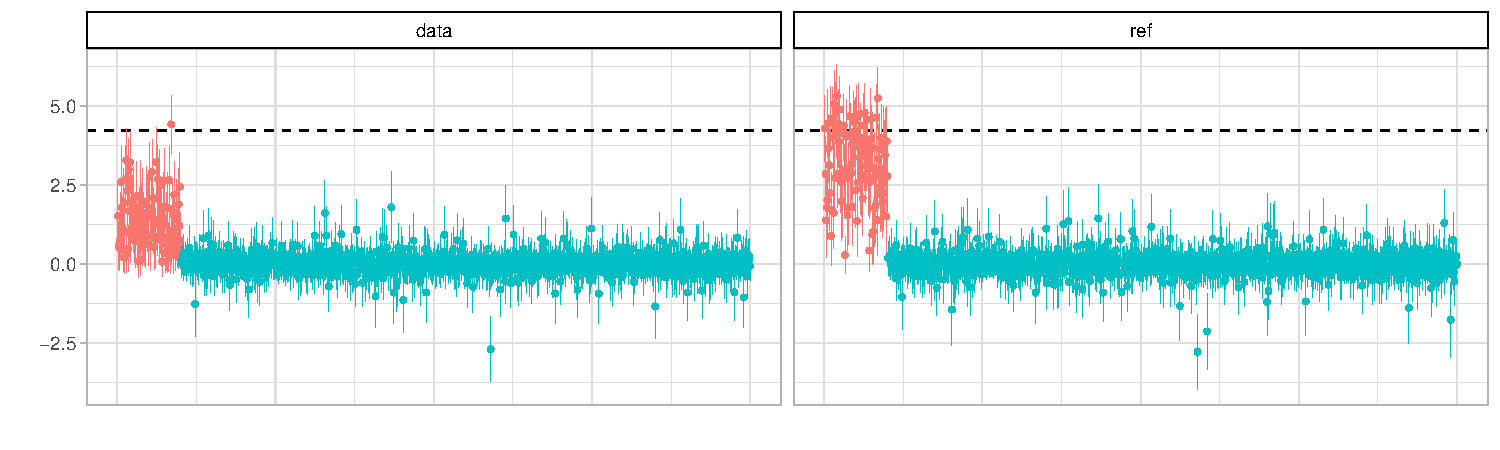
\includegraphics[width=0.98\textwidth]{graphics/post_int.pdf}
  \caption{Posterior intervals for the parameters of the normal means problem ($n=50$, $\rho=0.3$) using the regularised horseshoe prior. Posterior means and one standard deviation intervals depicted. Respectively in red and in blue relevant and non-relevant features. Horizontal dashed line corresponds to the true value of the mean for the relevant features.\\}
  \label{fig:posterior_intervals}
\end{figure}

Figure \ref{fig:posterior_intervals} shows an example of posterior distributions for the model \eqref{eq:normal_means_problem2} using the regularised horseshoe prior. Respectively on the right and on the left the results using or not the reference model approach. It is evident how the reference model helps in tearing apart the signals from the noise, resulting in less biased estimates. This is quantified in Figure \ref{fig:SESE_SSE} where average SESE and SSE are depicted after 100 simulations. We observe that the reference approach (in orange) has a clear lower error estimate for both the SESE and the SSE. As $n$ and $\rho$ grow, the amount of error diminish, as expected, due to a larger amount of information of the relevance of each variable provided by the data. We also note that the two priors seem to achieve very similar results, regardless of the approach used.

\begin{figure}[tp]
  \centering
  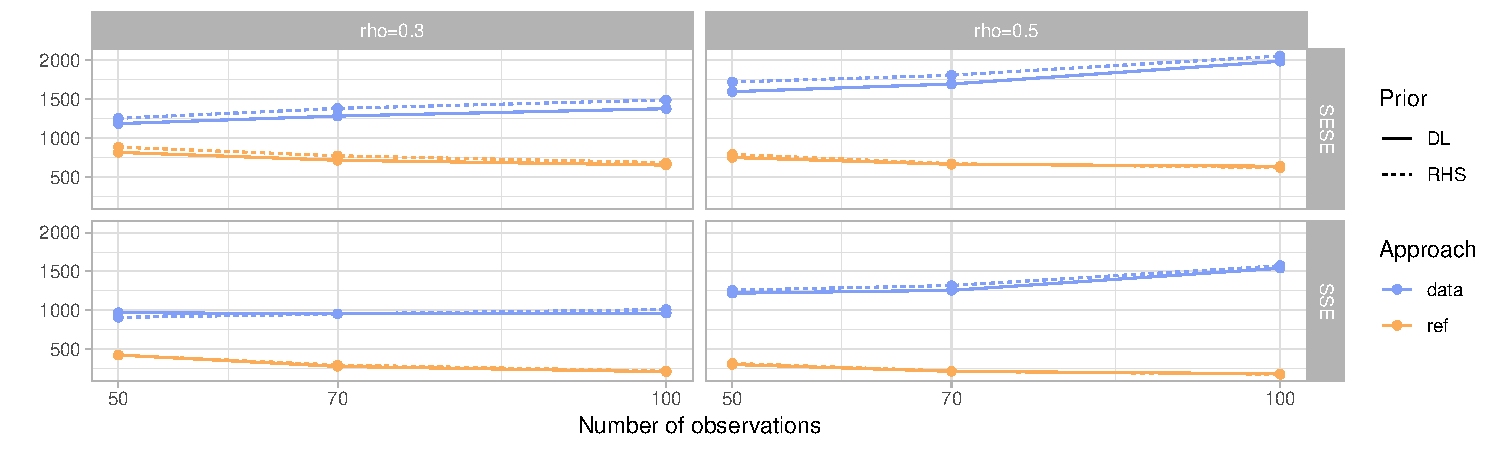
\includegraphics[width=0.98\textwidth]{graphics/SESE_SSE.pdf}
  \caption{Average SESE and SSE with one standard deviation error bars after 100 simulations.\\}
  \label{fig:SESE_SSE}
\end{figure}

Figure \ref{fig:k} shows the posterior means for the shrinkage factors of each parameter using the regularised horseshoe prior, averaged after 100 data simulations. Relevant and non-relevant features are respectively highlighted in red and blue. The ideal shrinkage would have $\kappa=0$ when the parameter is a signal, whereas $\kappa=1$ when it is noise. Respectively on the y-axis and on the x-axis are depicted the shrinkage factors using the reference model approach or not. If the reference model did not make any difference, we would expect the points to lie on the diagonal. Non-relevant features happen to lie on average on the diagonal for all the simulated scenario, meaning not evident benefits coming from the reference model. Although when considering the shrinkage amount for the relevant ones, we note that the points always lie under the diagonal, meaning that the reference model is able to shrink less the true signals. Such benefit is proportional to the difficulty of the problem, that is it increases with lower correlation and number of observations. Note that the perfect distinction of the two clusters of features (relevant and non-relevant) observable on both the marginal distributions of the shrinkage factors is due to the averaging over the 100 data simulations. In a single data realisation there would be more noise and the clusters would be closer and overlapping.
The results for the Dirichlet-Laplace prior are very similar and we do not include them in the paper.

\begin{figure}[tp]
  \centering
  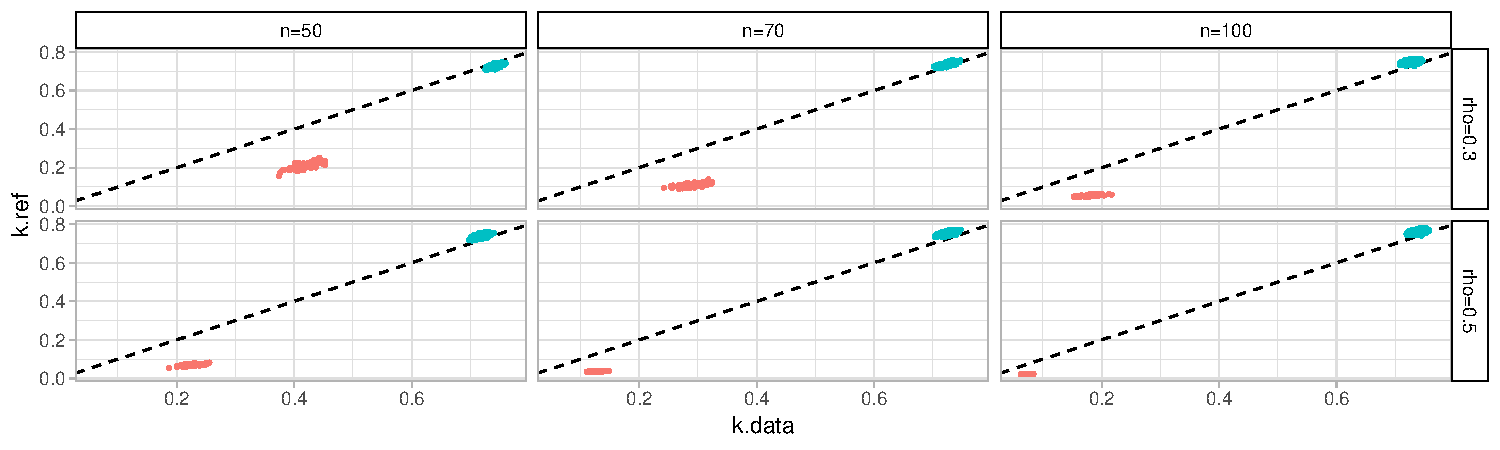
\includegraphics[width=0.98\textwidth]{graphics/k_RHS.pdf}
  \caption{Average posterior mean values for the shrinkage factors using the regularised horseshoe prior after 100 simulations. Respectively in red and in blue relevant and non-relevant variables.\\}
  \label{fig:k}
\end{figure}


\hypertarget{complete-selection}{%
\subsubsection{Complete selection analysis}\label{complete-selection}}
As complete selection procedures we consider the control of the local false discovery rate \citep{paper:efron, efron2012large}, the empirical Bayes median \citep{johnstone2004needles} and the selection by posterior credible intervals. 
\\
The control of the local false discovery rate is applied through the \texttt{R}-package \texttt{locfdr}. It consists in testing the z-values $\{z_{j}\}_{j=1}^{p}$ to belong to the theoretical null distribution $f_{0}$ (the null hypothesis, meaning no relevance) against the alternative hypothesis distribution $f_{1}$. In our case $f_{0}$ correspond to the standard normal distribution, see expression \eqref{eq:normal_means_problem2}. The quantity of interest is the local false discovery rate (loc.fdr) defined as:
\
\begin{equation}
loc.fdr(z)=P(H_{0}|z)=\frac{f_{0}(z)\pi_{0}}{f(z)}
\end{equation}
where $\pi_{0}$ is the prior probability of the null hypothesis and $f(z)=\pi_{0}f_{0}(z)+(1-\pi_{0})f_{1}(z)$ is the marginal distribution of the z-values. The latter is estimated using splines with 7 degrees of freedom and we select features with local false discovery rate under the value 0.2. Such a value is commonly suggested only because it corresponds to a Bayes factor large than 36 (assuming $\pi_{0}\geq0.9$), other values can be considered and in our experience do not affect the results of the comparison. We use the default setting to estimate $\pi_{0}$ from the data provided by the package.
\\
The empirical Bayes median procedure is given by the \texttt{R}-package \texttt{EbayesThresh} and consists in fitting a Bayesian model with a prior composed by a mixture of a delta in zero and a heavy-tailed distribution. We use, as suggested, a Laplace distribution resulting in a thresholding property, i.e. there exists a threshold value such that all the data under that threshold have posterior median equal to zero. Therefore the selection is done including those parameters whose posterior median is different from zero. The hyperparameter of the Laplace distribution and the mixing weight of the prior are estimated by marginal maximum likelihood. 
\\
The selection by posterior credible intervals is done using the regularised horseshoe prior and selecting those features whose posterior distribution does not include zero in the interval between the 0.05-th and the 0.95-th quantiles.


Figure \ref{fig:sensitivity_vs_fdr} reports the average sensitivity (on the y-axis) versus the average false discovery rate (x-axis) after 100 data simulations for the different combination of $n$ and $\rho$. For each method (different colours) the square and the circle dots respectively correspond to using or not the reference approach. The best selection performance is on the top-left corner of each plot, meaning lowest false discovery rate and highest sensitivity. It is possible to note that regardless of the method used, the use of a reference model improves the goodness of the selection diminishing the false discovery rate (left shifting) and/or augmenting the sensitivity (up shifting). In accordance with what expected, higher the number of observations and the correlation are, easier the selection is and, thus, the benefits of the reference model are less notable, since the unprocessed data already give enough information to identify the significant variables.

\begin{figure}[tp]
  \centering
  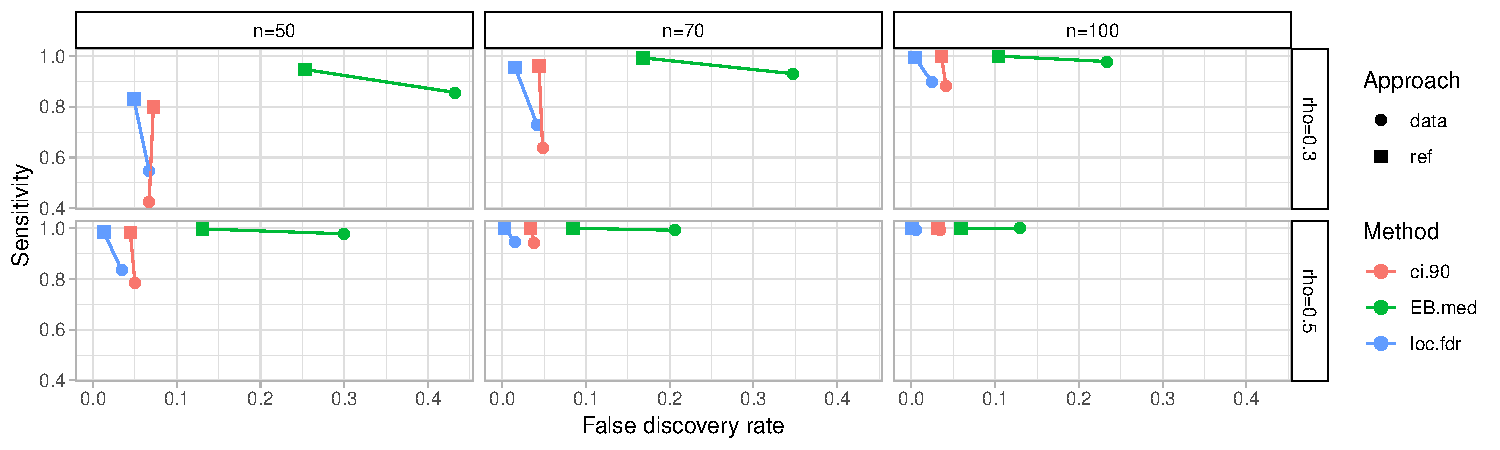
\includegraphics[width=0.98\textwidth]{graphics/sensitivity_vs_fdr.pdf}
  \caption{Sensitivity against false discovery rate after 100 data simulations.\\}
  \label{fig:sensitivity_vs_fdr}
\end{figure}

Figure \ref{fig:stability} shows the estimates of the stability measure proposed by \cite{paper:stability} with 0.95 confidence intervals after 100 simulations. Such a measure takes in account the variability of the subset of the selected features at each simulation (originally at each bootstrap sample), modelling the selection of each variable as a Bernoulli process. Further details are available in their paper as asymptotic normal distribution, based on which confidence intervals are computed. The reference model helps improving the stability of the selection: again, such benefit is notable when the problem is more difficult (small $n$ and $\rho$). We observe also less uncertainty in the stability estimates for the reference approach (i.e. the width of the 0.95 confidence intervals), which can be still connected to the overall stability of the procedure.

\begin{figure}[tp]
  \centering
  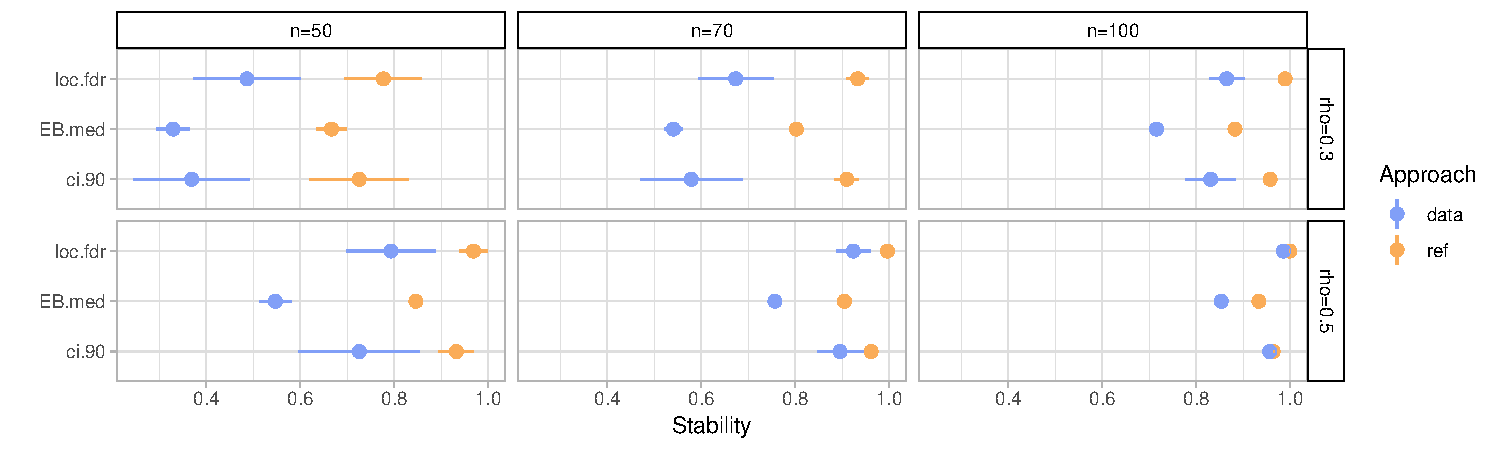
\includegraphics[width=0.98\textwidth]{graphics/stability.pdf}
  \caption{Stability estimates with 0.95 confidence intervals after 100 data simulations.\\}
  \label{fig:stability}
\end{figure}




\hypertarget{real-world-data}{%
\subsection{Real world data: the body fat dataset}\label{real-world-data}}

We conclude our experiments using one more time the real world dataset body fat, already described in the comparison between the projection predictive approach and the stepwise regression in Section \ref{projection}. We carry out two different analyses: one using the normal means problem framework and the other one using the stepwise backward regression. In the former, we add to the original data noisy uncorrelated covariates up to a total of 1000 features. These covariates are normally distributed and scaled as the original ones. We compute correlations between each variable and the target variable, that is the amount of fat, and transform them by Fisher transformation. The original assumption, in order that \eqref{eq:fisher_transformation} holds, is that the variables are jointly normally distributed. In our experience the normal approximation in \eqref{eq:fisher_transformation} is still reasonable, but after rescaling by $\sqrt{n-3}$ we do not fix the variance to be one, instead we estimate it from the data. The methods we compare are those used in Section \ref{complete-selection}: the control of the local false discovery rate (loc.fdr), the empirical Bayes median (EB.med) and the selection by posterior credible intervals at level 0.9 (ci.90). The maximum likelihood estimator is used to estimate the variance of the null hypothesis in the local false discovery rate \cite[see][Chap. 6]{efron2012large}, whereas the median absolute deviation from zero for the empirical Bayes median method. The selection via posterior credible intervals is done using a regularised horseshoe prior on the parameters for the means, while a standard log-normal  prior for the variance. In order to vary the difficulty of the selection, we bootstrap subsamples of different sizes, going from $n=50$ up to $n=251$. Each time results are averaged over 100 bootstrap subsamples.

\begin{figure}[tp]
  \centering
  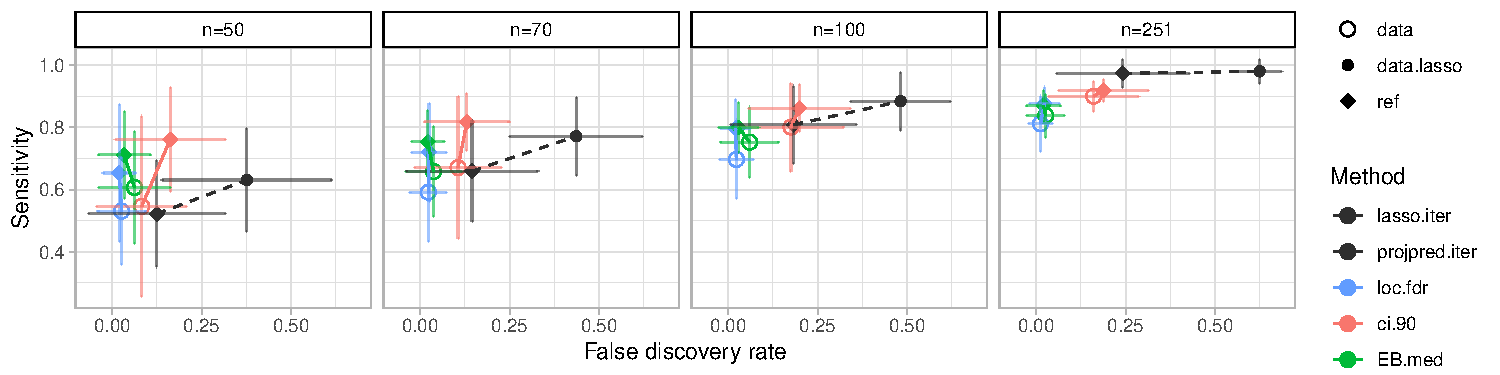
\includegraphics[width=0.98\textwidth]{graphics/bodyfat_sensitivity_vs_fdr.pdf}
  \caption{Sensitivity against false discovery rate after 100 bootstrap samples.\\}
  \label{fig:bodyfat_sensitivity_vs_fdr}
\end{figure}

\begin{figure}[tp]
  \centering
  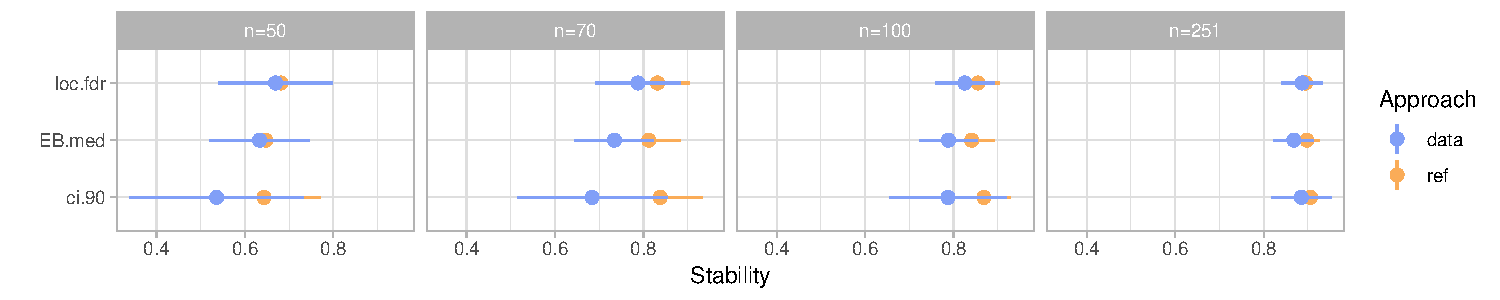
\includegraphics[width=0.98\textwidth]{graphics/bodyfat_stability.pdf}
  \caption{Stability estimates with 0.95 confidence intervals after 100 bootstrap samples.\\}
  \label{fig:bodyfat_stability}
\end{figure}

Figure \ref{fig:bodyfat_sensitivity_vs_fdr} shows the sensitivity against the false discovery rate. Since we do not have a ground truth regarding the original covariates of the data, we believe it is reasonable to consider all of them relevant, at least at some degree. We thus consider as non-relevant all the artificially added ones. In almost all the bootstrapped subsamples, the reference model improves both in terms of sensitivity and false discovery rate. When $n=50$, we observe a worsening in terms of false discovery rate, yet in a lower amount compared to the gain in sensitivity.  We observe again that the benefits are more evident as the selection is more challenging (i.e. less number of observations). Figure \ref{fig:bodyfat_stability} shows the stability results, still using the measure provided by \cite{paper:stability}. The benefits of the reference model are here marginal: small improvements can be observed, but overall not very notable.

%\begin{figure}[tp]
%  \centering
%  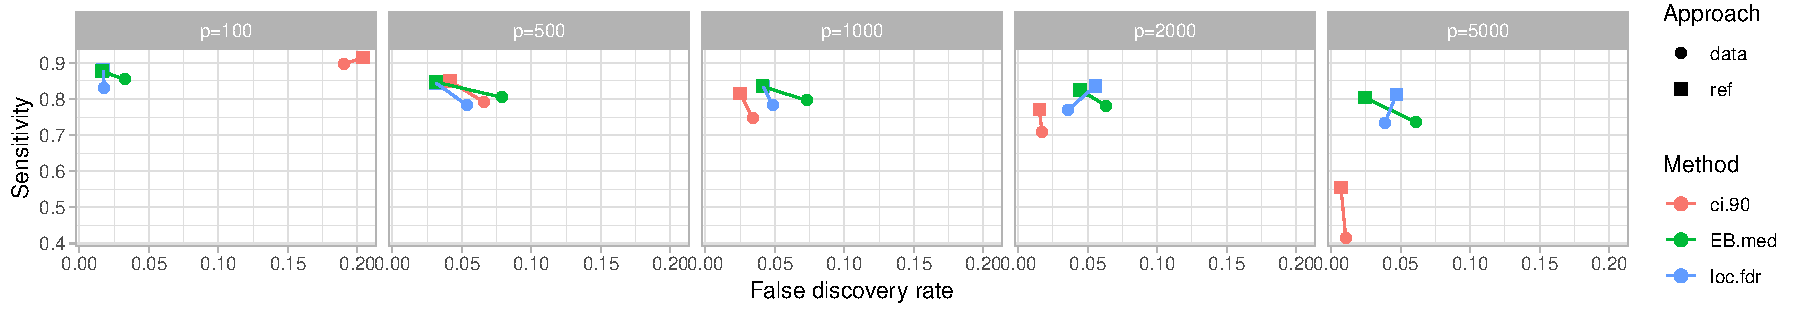
\includegraphics[width=0.98\textwidth]{graphics/bodyfat_varyingP_sensitivity_vs_fdr.pdf}
%  \caption{Sensitivity against false discovery rate after 100 data simulations.\\}
%  \label{fig:bodyfat_varyingP_sensitivity_vs_fdr}
%\end{figure}

%\begin{figure}[tp]
%  \centering
%  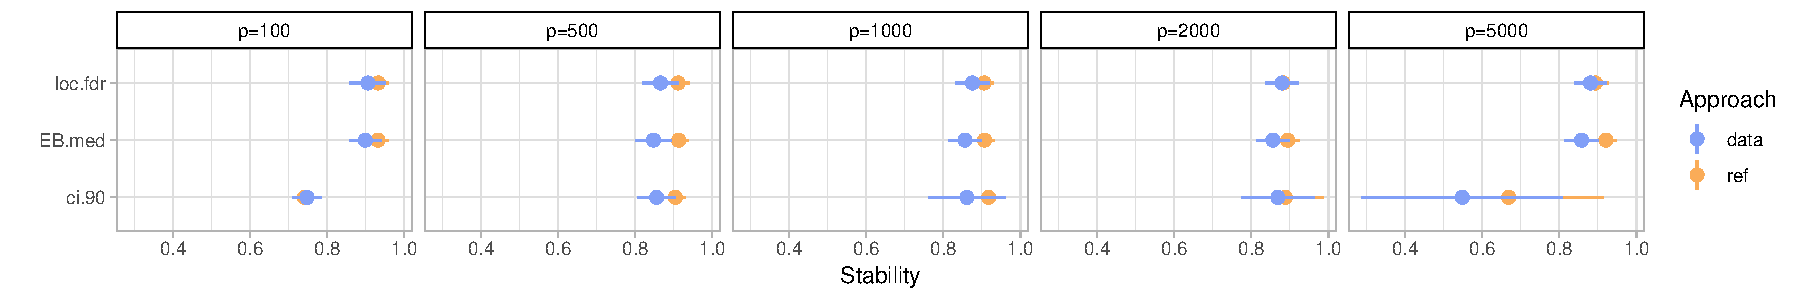
\includegraphics[width=0.98\textwidth]{graphics/bodyfat_varyingP_stability.pdf}
%  \caption{Stability estimates with 0.95 confidence intervals after 100 data simulations.\\}
%  \label{fig:bodyfat_varyingP_stability}
%\end{figure}

% As an additional experiment, we run the selection bootstrapping from the whole dataset, but varying the overall number of covariates from $p=100$ up to $p=5000$. Figures \ref{fig:bodyfat_varyingP_sensitivity_vs_fdr} and \ref{fig:bodyfat_varyingP_stability} respectively show the sensitivity against the false discovery rate and the stability results. As in the previous experiment, we note that the reference model has a larger impact as the complexity of the problem increases: previously as $n$ decreases, now as $p$ increases. Note the different scale of the sensitivity and the false discovery rate axes. We observe an odd behaviour of the selection via credible intervals (ci.90): when $p=100$ and $p=5000$ the results are strongly different from the other methods, both in terms of sensitivity/false discovery rate and stability. 
%Such behaviour can be in part explained by the connection between low stability and high uncertainty in the estimates.

\begin{figure}[tp]
  \centering
  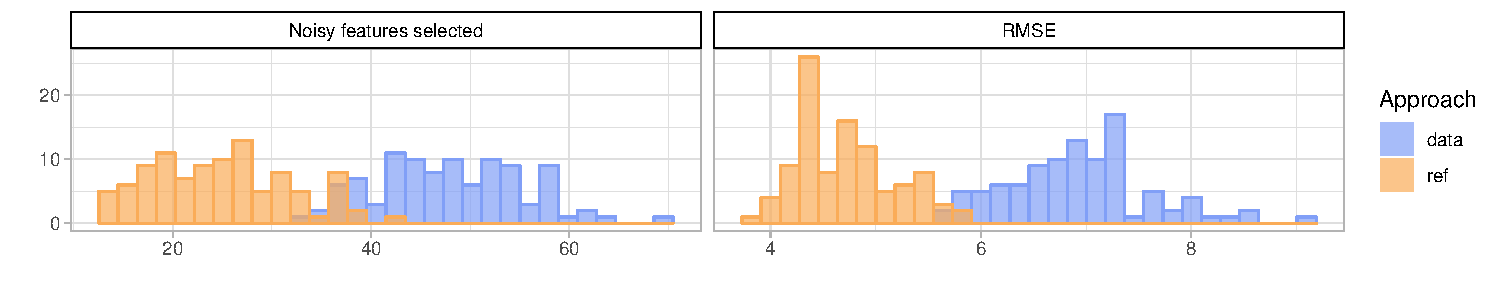
\includegraphics[width=0.98\textwidth]{graphics/bodyfat_step_refvsdata.pdf}
  \caption{Stepwise backward selection using or not the reference model: number of noisy feature included in the model and RMSE after 100 bootstrap samples.\\}
  \label{fig:bodyfat_step_refvsdata}
\end{figure}

In the second analysis, we repeat the selection of Section \ref{projection} via stepwise backward regression by AIC. In this case the overall number of covariates (original plus noisy) is 100, as it was in the last part of Section \ref{projection}. We compare results using or not the reference model on top of the procedure according to our simple reference model approach; here the reference model is again given by the first five supervised principal components. Figure \ref{fig:bodyfat_step_refvsdata} shows the number of noisy features included in the final model and the out-of-sample root mean square error (RMSE). Results are after 100 bootstrap samples on the whole dataset, and the predictive performance is tested on the observations excluded at each bootstrap sample. We observe that the reference model reduces the number of noisy features included in the final model. This leads to less overfit to the data and, thus, improved out-of-sample predictive performance in terms of RMSE. Also in this case, we see that there is not a notable difference in terms of the stability of the two approaches, which in this case is qualitatively assessed through the variability of the histogram. We can not use the stability measure provided by \cite{paper:stability}, since it does not take in account possibly swaps in the set of selected features due to high correlation between the covariates, which in this case can occur. Our reference model approach applied to the stepwise backward regression achieves outstanding improvements considering its simplicity, yet it does not reach the goodness of more thoughtful implementations, as projpred (see results of Section \ref{projection}). 

We would like the reader to note that in this example we have still used the reference model defined as a linear regression over some supervised principal components, because of its fairly good predictive performance and speed to fit. We do not argue that this is always a good choice, more sophisticated and well-thought models can lead to even better results. Since in our case the sake of the analysis was only explanatory in terms of the comparison we have been carrying out through the paper and needed to average results over many (100) simulations, we preferred to stick to such model.




\hypertarget{conclusion}{%
\section{Conclusion}\label{conclusion}}

This paper has discussed the importance of using a reference model when dealing with feature selection, or more in general model reduction. We want to highlight that the goal of this paper is not to provide a specific algorithm or procedure to carry out the selection, but rather to bring motivations and attentions to the general use of a reference model. 
\\
The reference model acts as an approximation of the data generation mechanism through its predictive distribution. Such approximation is generally less noisy than the sample estimation available from the observed data, leading to the main benefits of the reference model approach. In our comparisons, we have analysed the effect of a reference model in the form of a filter on the observed target values on top of different variable selection methods widely used. The overall benefits we have showed independently of the specific method applied, consisting in stability and goodness of the selection, motivate what we refer to as the reference model approach for the model reduction framework. Such approach translates into a family of different methods, some of which have been present in the literature for several years.
\\
In a real-world data application (body fat data), we have applied one of these methods, namely the projection predictive approach as indicated by \cite{paper:projpred}, in opposition to the selection via stepwise backward regression with the results provided by \cite{paper:bodyfat}. The selection via projection resulted to be more stable and led to a sparser representation. After adding additional noisy covariates, the selected submodel showed also higher predictive performance compared to the one selected by the stepwise backward regression, which included several non-relevant features. Applying a reference model on top of the stepwise backward regression resulted in a minor number of non-relevant features selected and an improved predictive performance, yet without reaching the projection predictive approach results.
\\
Whenever it is possible to come up with a reasonable reference model, our suggestion is to employ it when selecting models, because of its nature as baseline of the comparisons and its ability to improve the selection. Note that one of the main challenges in many real world application will consist in devising the reference model itself and assessing its predictive performance, for which we suggest the user to rely on robust modelling workflow indications \cite[see e.g.][]{gabry2019visualization}.
\\
All Bayesian models have been implemented using \texttt{Stan} \citep{paper:stan}, which uses HMC-NUTS sampler \citep{hoffman2014no} and allows full posterior Bayesian inference. The code to run all the experiments is available at \url{https://github.com/fpavone/ref-approach-paper}. 




 
\bibliography{ref_approach}

%\appendix

%\hypertarget{ap:shrinkage_signal}{%
%\section{Appendix: Shrinkage factors with Dirichlet-Laplace prior}\label{ap:shrinkage_signal}}
%Figure \ref{fig:k_DL} shows the posterior mean shrinkage factors using the Dirichlet-Laplace prior for the normal means problem in the simulated data study of Section \ref{comparison}. The result is qualitatively equal to the regularised horseshoe prior's one (see Figure \ref{fig:k}). 

%\begin{figure}[tp]
%  \centering
%  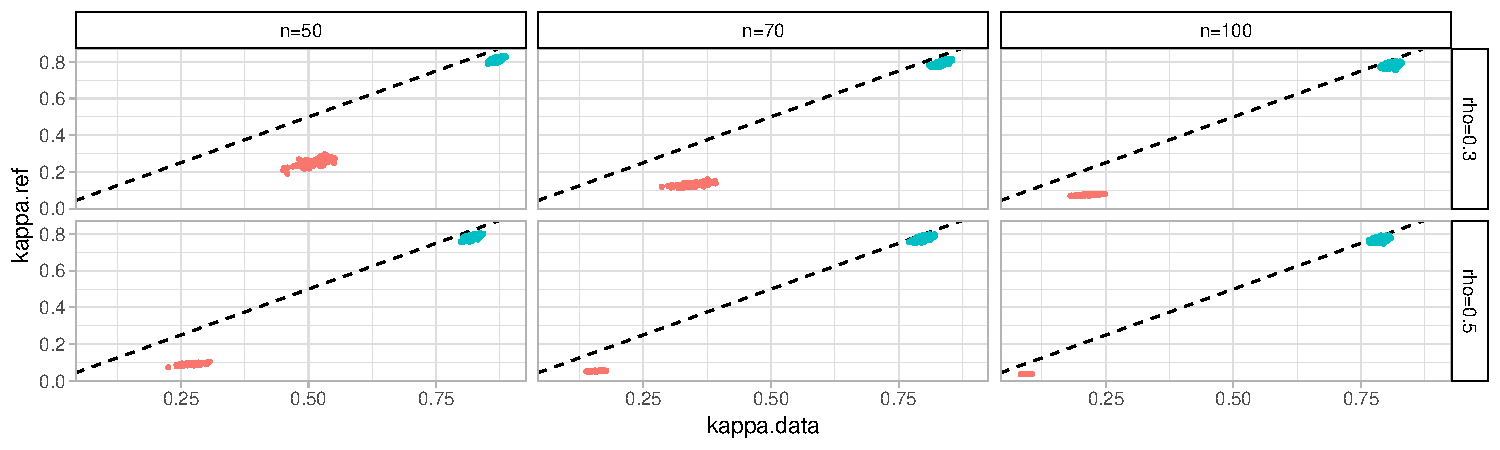
\includegraphics[width=0.98\textwidth]{graphics/k_DL.pdf}
%  \caption{Average posterior mean values for the shrinkage factors using the Dirichlet-Laplace prior after 100 simulations. Respectively in red and in blue relevant and non-relevant variables.\\}
%  \label{fig:k_DL}
%\end{figure}


\end{document}







